\documentclass[a4paperm]{article}
%\documentclass[12pt,twocolumn]{article}

\usepackage[T2A]{fontenc}
\usepackage[utf8]{inputenc}
\usepackage[russian,english]{babel}
\usepackage{amsmath,amsthm,amssymb,stackrel}
\usepackage[affil-it]{authblk}
\usepackage{cite}
\usepackage{scrextend}
\usepackage{verbatim}
\usepackage{paralist}
\usepackage[mediumspace,mediumqspace,Grey,squaren]{SIunits}
\addtokomafont{labelinglabel}{\sffamily}
\usepackage{amsmath}
\usepackage{graphicx}
 \usepackage[usenames, dvipsnames]{color}
 \usepackage{multirow}
 \usepackage{longtable}
 \usepackage{lineno}
 
 \usepackage{xr}
 
 
%\usepackage[none]{hyphenat} %no nyphenation

\usepackage{SIunits}
\usepackage{miller}
\usepackage[version=3]{mhchem}

\usepackage{float} %H with figures

\setlength{\parindent}{5ex}

 \usepackage{newfloat} %For numbering of supplemmentary figures
 \DeclareFloatingEnvironment[name={Supplementary Figure}]{suppfigure}

\graphicspath{{figures/}}
\externaldocument{supplementary/smose_supp}


\begin{document}

%\linenumbers

\title{New crystal structures of the transition metall dichalcogenides}


\author[1,2]{Pavel N. Gavryushkin
   \thanks{Electronic address: \texttt{gavryushkin@igm.nsc.ru, p.gavryushkin@g.nsu.ru}; Corresponding author}}     
\author[1]{Nursultan Sagatov}
\author[3]{Zakhar I. Popov}

\affil[1]{Sobolev Institute of Geology and Mineralogy, Siberian Branch of Russian Academy of Sciences, prosp. acad. Koptyuga 3, 630090 Novosibirsk, Russian Federation}
\affil[2]{Novosibirsk State University, Pirogova 2, Novosibirsk 630090, Russian Federation}
\affil[3]{ИБХФ}

\date{}
\maketitle

%\linenumbers

\begin{abstract}
\begin{enumerate}
	\item Проведены предсказания и обнаружено несколько новых  структур, существенно отличащихся от ранее известных H и T 
	\item Предсказанные структуры характеризуются динамической стабильностью, однако энтальпии их образования выше энтальпий H и T структур.
	 \item С помощью автоматизированных топологических алгоритмов проведён поиск топологических аналогов. Все структуры, включая fxt и fes характеризуются уникальными топологическими типами и не имеют структурных аналогов в ICSD. Исключение составляет horH структура, характеризующаяся той же топологией, что и T-структура. 
\end{enumerate}
\end{abstract}

%%%%%%%%%%%%%%%%%%%%%%%%%%%%%%%%%%%%%
\section*{Introduction}
%%%%%%%%%%%%%%%%%%%%%%%%%%%%%%%%%%%%%
Transition metall dichalcogenides (TMD) crystallise in four main structural types: CdI2, MoS2, FeS2 (pyrite-type and less frequently marcasite-type).
Fisrt two structural types are characterised by the layered structures with Ch-TM-Ch (Ch--chalcogenide, TM--transition metall) sandwiches bonded to each other by the weak Van-der-Waals bonds. 
These quasi-2D sandwiches attract considerable attention due to their semiconducting, superconduting and magnetic properties.
In particular, 2D layers of MoS2, WS2, MoSe2, WSe2, and MoTe2 have a direct band gap and can be used as transistors and due to the strong spin-orbit coupling are perspective spintronics.
Due to trigonal and hexagonal symmetry of the separate sandwich-lyers produced from MoS2 and CdI2 structures, they can be designated as 1H and 1T respectively, according to Ramsdell notation.  


The top-layer of sulphur in the the sandwich of MoS2 was successfully changed on the layer of Se with the formation of the so-called Janus SMoSe structure  \cite{lu2017}.
In the present work we investigate stability and energy of Janus structures sufficiently different in geometry and topology from T and H structures.
Using topological anlysis, we analyse uniquness of the found structures and acess possibility of their experimental synthesis.
Preliminary calculations of the electronic structures shows that some of the found structures are direct band gap semiconductors (Захар, поправь меня, если я не прав).
The special paper will be devoted to the results of these calculations.


\subsubsection*{Crystal structures of MCh2, M=Mo,W,Vm, Ch=S,Se}
At ambient conditions MoS2, WS2, MoSe2, WSe2 crystallise in the arche-type molibdenite (MoS2) structure.
In these structure atoms of chalcogenes form close-packed layers placed exacly one under another along c-axis.
TM atoms occupy center of trigonal prismatic cavities between the layers.
Different stacking of such a 2D layers produce different polytypes.
If the repition stacking is reprpoduced through each two layers the structure has hexagonal symmetry and according to Ramsdell notation is denoted as 2H-polytype. 
As in the present manuscript, we consider only isolated 2D-layers, we will designate them as H-layers.

If the layers of chalcogene atoms are shifted such that the top-layere is placed in triangular holes, the coordination polyhedron changes from trigonal prism to octahedron and archetype CdI2 structure is formed. 
Due to trignaly symmetry of sandwich-layers of such a structure, they can be designated as T-layers.

The 1T structure for TMCh2 compounds, where TM=Mo, W, and V, and S, Se, and Te are less energetically favourable than 2H structres of the same compoistion.
However, these 1T structures can be stabilised by the impurities of Li atoms or by some deformations (Захар, добавь тут ссылку).

V is different from W and Mo in that it does not produce dichalcogenides at ambient conditions.
VSe2 is known in the form 2H structure with additional V adoms in the centers of empty trigonal prisms in between the sandwiches and composition Se2V1.005

Comment. 
fes structure denoted as S-MS2 in \cite{tang2021_smose}, from square.
fxt structure denoted as H' in \cite{ma2016_h'}.
Similarly there is T' – deformed T-phase.
We can follow this notation, designating our phases by symmetry with addition of '.

%%%%%%%%%%%%%%%%%%%%%%%%%%%%%%%%%%%%%
		\section{Methods}
%%%%%%%%%%%%%%%%%%%%%%%%%%%%%%%%%%%%%
The search for the lowest-enthalpy structures of XMY were performed using evolutionary algorithms implemented in the USPEX package \cite{uspex1,uspex2,uspex3} and the random sampling method implemented in the AIRSS software \cite{airss1,airss2} at 50, 100, 200, 300, and 400 GPa.

The search with USPEX was performed in fixed composition mode with 2--6 formula units per unit cell.
The size of the first generation in the calculations was equal to 180 structures.
50\% of the structures with the lowest enthalpy were selected after the optimization and then used to produce the next generation.
A new generation was produced as follow: 50\% of all structures were generated by heredity, 10\% -- by atomic mutation, 10\% –- by lattice mutation, and 30\% –- randomly.
In average, 40--47 generations have been produced and relaxed.
Using AIRSS, about 5000--6000 structures were randomly generated and optimized for compounds with 4 and 6 formula units per unit cell, and those with the lowest enthalpy were selected.

The total energies and forces were calculated by solving the Schr\"{o}dinger equation based on projector augmented plane-wave implementation of density functional theory (DFT) using the VASP package \cite{vasp1,vasp2}.
Exchange correlation effects were treated in the generalized gradient approximation (GGA) with Perdew-B\"{u}rke-Ernzerhof scheme \cite{pbe}.

In all crystal structure prediction calculations, medium-quality optimization was performed using the conjugate gradient method.
The medium quality settings were as follows: plane-wave cutoff energy --- 420 eV; Monkhorst-Pack k-point sampling grid of spacing --- 0.5 \AA$^{-1}$; Gaussian smearing with parameter $\sigma$ = 0.15 eV.
The most promising predicted structures were then optimized at various pressures with higher accuracy: the cutoff energy --- 700 eV, k-point sampling grid of spacing --- 0.2 \AA$^{-1}$, and $\sigma$ = 0.05 eV.

To study a dynamic stability of predicted structures phonon spectra were calculated with the PHONOPY code \cite{phonopy}.


%%%%%%%%%%%%%%%%%%%%%%%%%%%%%%%%%%%%%
			\section{Results}
%%%%%%%%%%%%%%%%%%%%%%%%%%%%%%%%%%%%%

\subsection{Similarity and differences of H, T, fxt and fes structures}

Although H and T structures are charactersied by the different coordination polyhedrons, they are similar in the manner of their interconnection.
H structure consists of trigonal prisms MoS6 (MoS3Se3 for Janus structures), and T structure – of the octahedra of the same composition (Figure\ref{1H1T}).
Each trigonal prism share all three vertical edges with the neighboring prisms and does not share any faces.
As the result each vertice and each verical edge of the trigonal prism is common for three prisms (Figure \ref{1H1T}).
Similarly in T structure, each octahedron share all edges inclined to the plane of sulphur atoms with neighbouring octahedra, and each vertice is common for three octahedra (Figure \ref{1H1T}).
Bond valence of Mo--S bond is nearly equal to +4/6 and there are necessary three such a bonds to compensate negative charge of 2$^-$i of the suphur atom.
The interconnection through the edges but provides the longer distance between high-chargeed Mo4+ ions in comparison with interconnection through the faceing, thus reducing the energy of Couloumb interaction.

The recently found fes and fxt structures are also charactersied by the trigonal prosmatic coordination.
However, in these structure prisms are connected not only through edges but also through the faces.
The whole structure can be constructued from the two edge-connected trigonal prisms (Figure \ref{2prism_oct}b).
As the result, the enthalpis of fxt and fes structures are higher than that of H structure, in full accordance with the Pauling rule \cite{Pauling1929}.
In fxt and fes structures, as well as in H and T structures, each at sulphur are connected to three Mo atoms in fxt and fes structure, providing the local charge balance.

H and T structures provide the most homogenic distribution of sulphur and Mo atoms. 
Both Mo and S nets consists of the geometrically equal triangular loops.
Eadge-sharing interconnection of trigonal prisms realised in fxt and fes structures inevitably results in the appearance of the cavities bigger than that in H and T structures. 
In fes structure the cavities have the form of the slightly compressed cube (Figure \ref{fes_SMoSe}).
The volume of these cavities is almost two times larger than the volume of the cavities in H structure (38.8 against 17.7 \AA$^3$).
In casse of fxt structure, the volume of hexagonal cavities (Figure \ref{fxt_SMoSe} is almost 8 times larger than in H structure (137.8 against 17.7 \AA$^3$).
In contrast to trigonal prisms, the face-sharing of the right octahedra seems to be problematic for quasi 2D structure, as it is results in the deviation from the flat arrangement (Figure\ref{2prism_oct}b).
However, as it will be shown below, the dynamically stable structures with face sharing deformed octahedra can be also produced. 


\begin{figure}[H]
        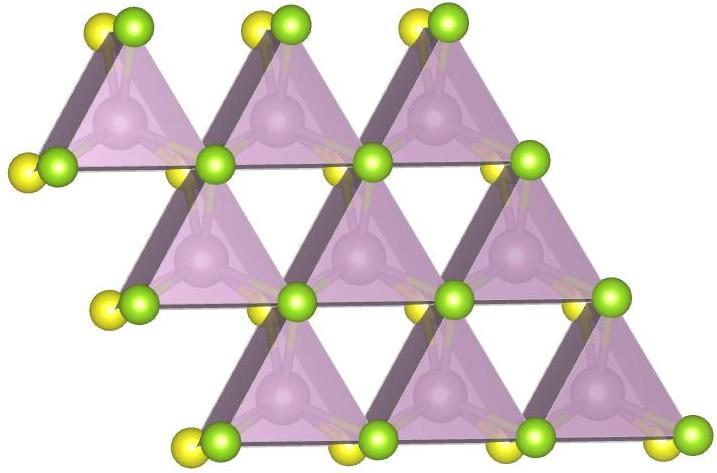
\includegraphics[width=0.4\textwidth]{1H.jpg}
        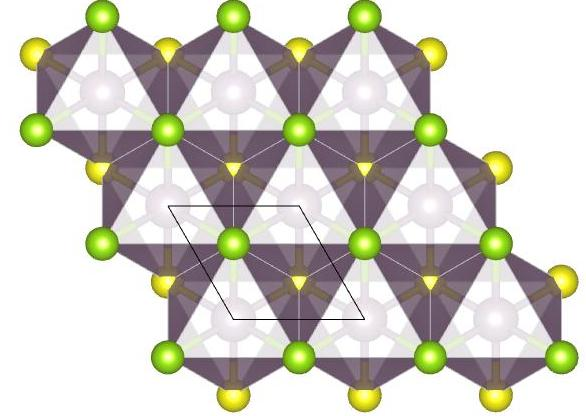
\includegraphics[width=0.4\textwidth]{1T.jpg}
        \caption{Packing of trigonal prisms and octahedra in H and T structures}
\label{1H1T}
\label{fes_fxt}
\end{figure}

\begin{figure}[H] \centering
	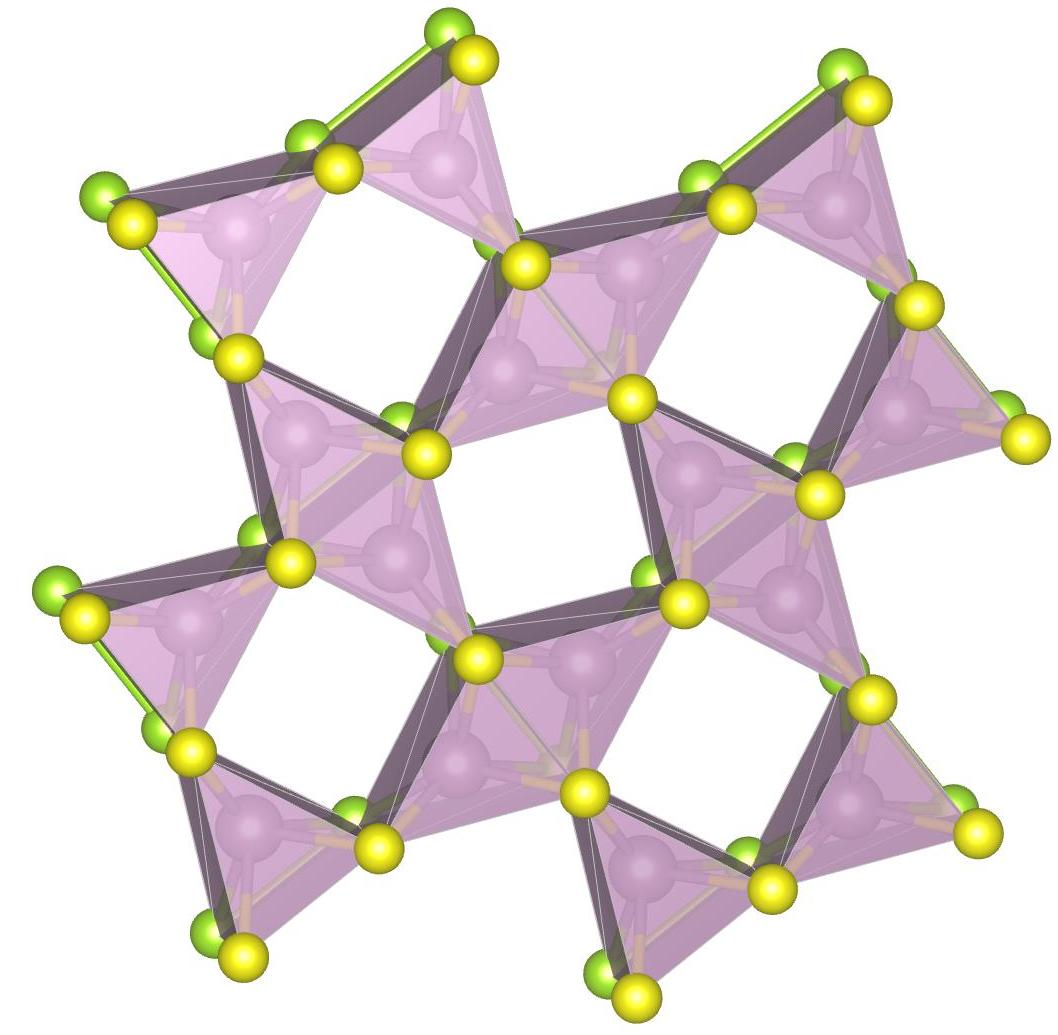
\includegraphics[width=0.4\textwidth]{fes_SMoSe.jpg}
        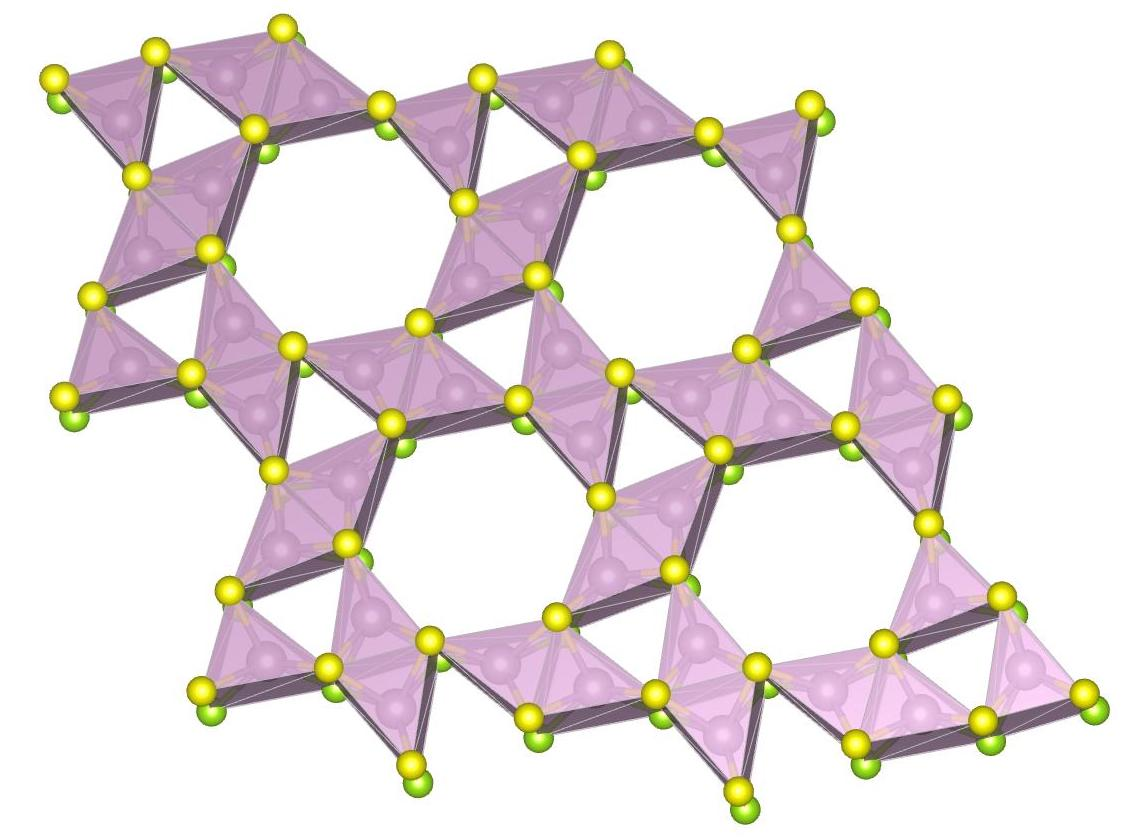
\includegraphics[width=0.5\textwidth]{fxt_SMoSe.jpg}
	\caption{Packing of trigonal prisms in fes and fxt structures.}
\label{fes_fxt}
\end{figure}

\begin{figure}[H] \centering
	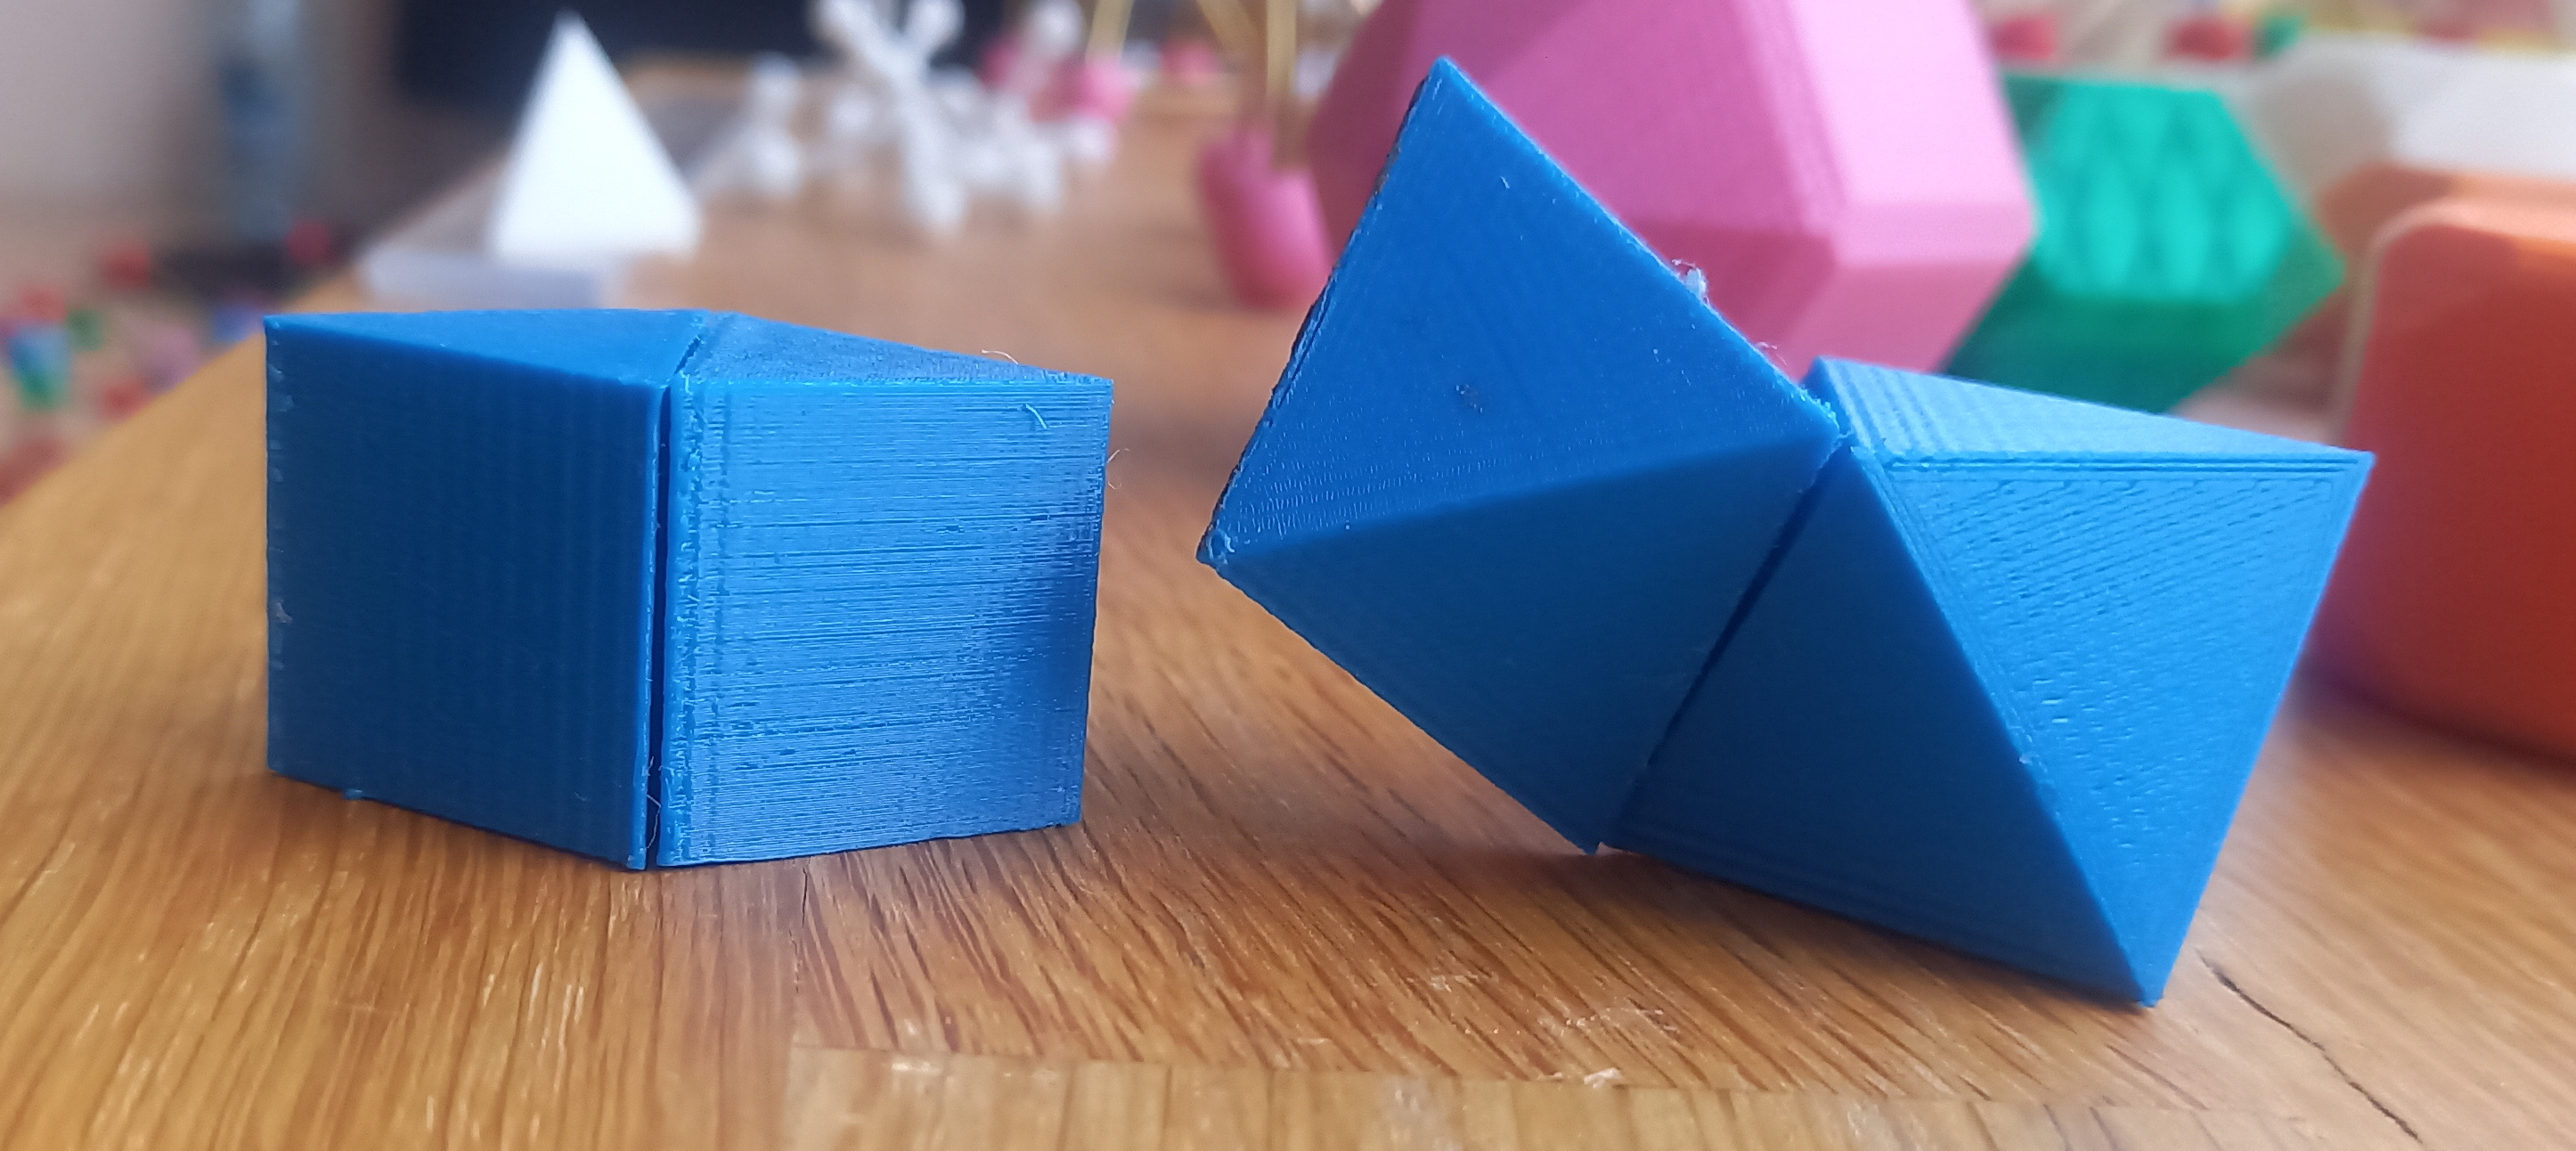
\includegraphics[width=0.5\textwidth]{2prism_oct.jpg}
	\caption{Two face-shared trigonal prisms and octahedra, the diviation from the horisontal plane in the last case is clearly visible}
\label{2prism_oct.jpg}
\end{figure}


%%%%%%%%%%%%%%%%%%%%%%%%%%%%%%%%%%%%%
		\subsection{The new crystal structures}
%%%%%%%%%%%%%%%%%%%%%%%%%%%%%%%%%%%%


%%%%%%%%%%%%%%%%%%%%%%%%%%%
\subsubsection{Structures with trigonal prismatic coordination}
%%%%%%%%%%%%%%%%%%%%%%%%%%

To compare topologies of H, fes, and fxt structures and produce similar structures with trigonal prismatic coordination, we present the structures as different fillings of the hexagonal net of sulphur atoms (Figure \ref{H-based}).
H-structure presents the most symmetric chess-board-like filling.
The fes structure can be also considered as the chess-board filling, but with doubled triangular cell, having the form of rhombuses.
After optimisation these rhombuses trasforms in the right squares.
In fxt structure the non-filled loops are of two types.
The first are three doubled triangular (rhombuses) connected through the faces, having the form of right hexagons.
The second are primitive triangles.
The optimisation does not sufficiently change the form of the non-filled loops, only slightly deforming hexagons.


Three new structures were produced by means of the filling of triangles in the hexagonal net of the sulphur atoms.
We name them abstractly test1, test2, and test3.
We failed to produce new structures obeying the local charge balance, i.e. the structures in which each vertice of the trigonal prism would be common for two other prisms.
In the structure test1, each sulphur atom is common for two or four filled prisms, in test2 and test3 – for 2, 3, and 4 (Figure \ref{H-based}).
Test3 structure is different from the other structures in that it characterised by the presence of trigonal prisms with two common faces, while in all other structures prisms has no more than one common face.
Optimisation of test3 structure sufficiently affect the arrangement of sulphur atoms.
In the final structure the net of sulphur atoms is not more the hexagonal one.

Presense of common edges and faces of [MoO6] trigonal prisms in fxt, fes, test1, test2, and test3 structure results in shorter Mo--Mo distances in comparison with 1H structure, where prisms have only common edges.
In H structure, Mo atoms form regular hexagonal net with all Mo--Mo bonds being equal to 3.25 \AA.
In fxt, fes, test1, test2, and test3 structures Mo--Mo distances varie in some range, with formation of Mo--Mo dimer connected by the stronger bonds.
In optimised H structure, the Mo--Mo bonds distances are equal to 3.25 \AA, in H-hor it reaches 3.08 \AA, in test1 -- 2.9 \AA, in fxt, fes, and test2 -- in average 2.62 \AA, and test3 is characterised by the shortest Mo--Mo distance of 2.22 \AA length. 
The dimers are in turn connected in chains and layers by the weaker bonds.

Comment. fxt structure was considered as grain-boundary structure of H structure. Similarly we can describe test-1 and test-2 structure, as structures forming at grain boundary forming at contact of grains growing in oppoiste direction (horizontal direction on the figure).
Comment. Considering the fact that the total energies of the H phase are comparable to those of the T phase it is reasonable to expect that our proposed H structure could be found at least with the same probability as the T configuration.

\begin{figure}[H] \centering
        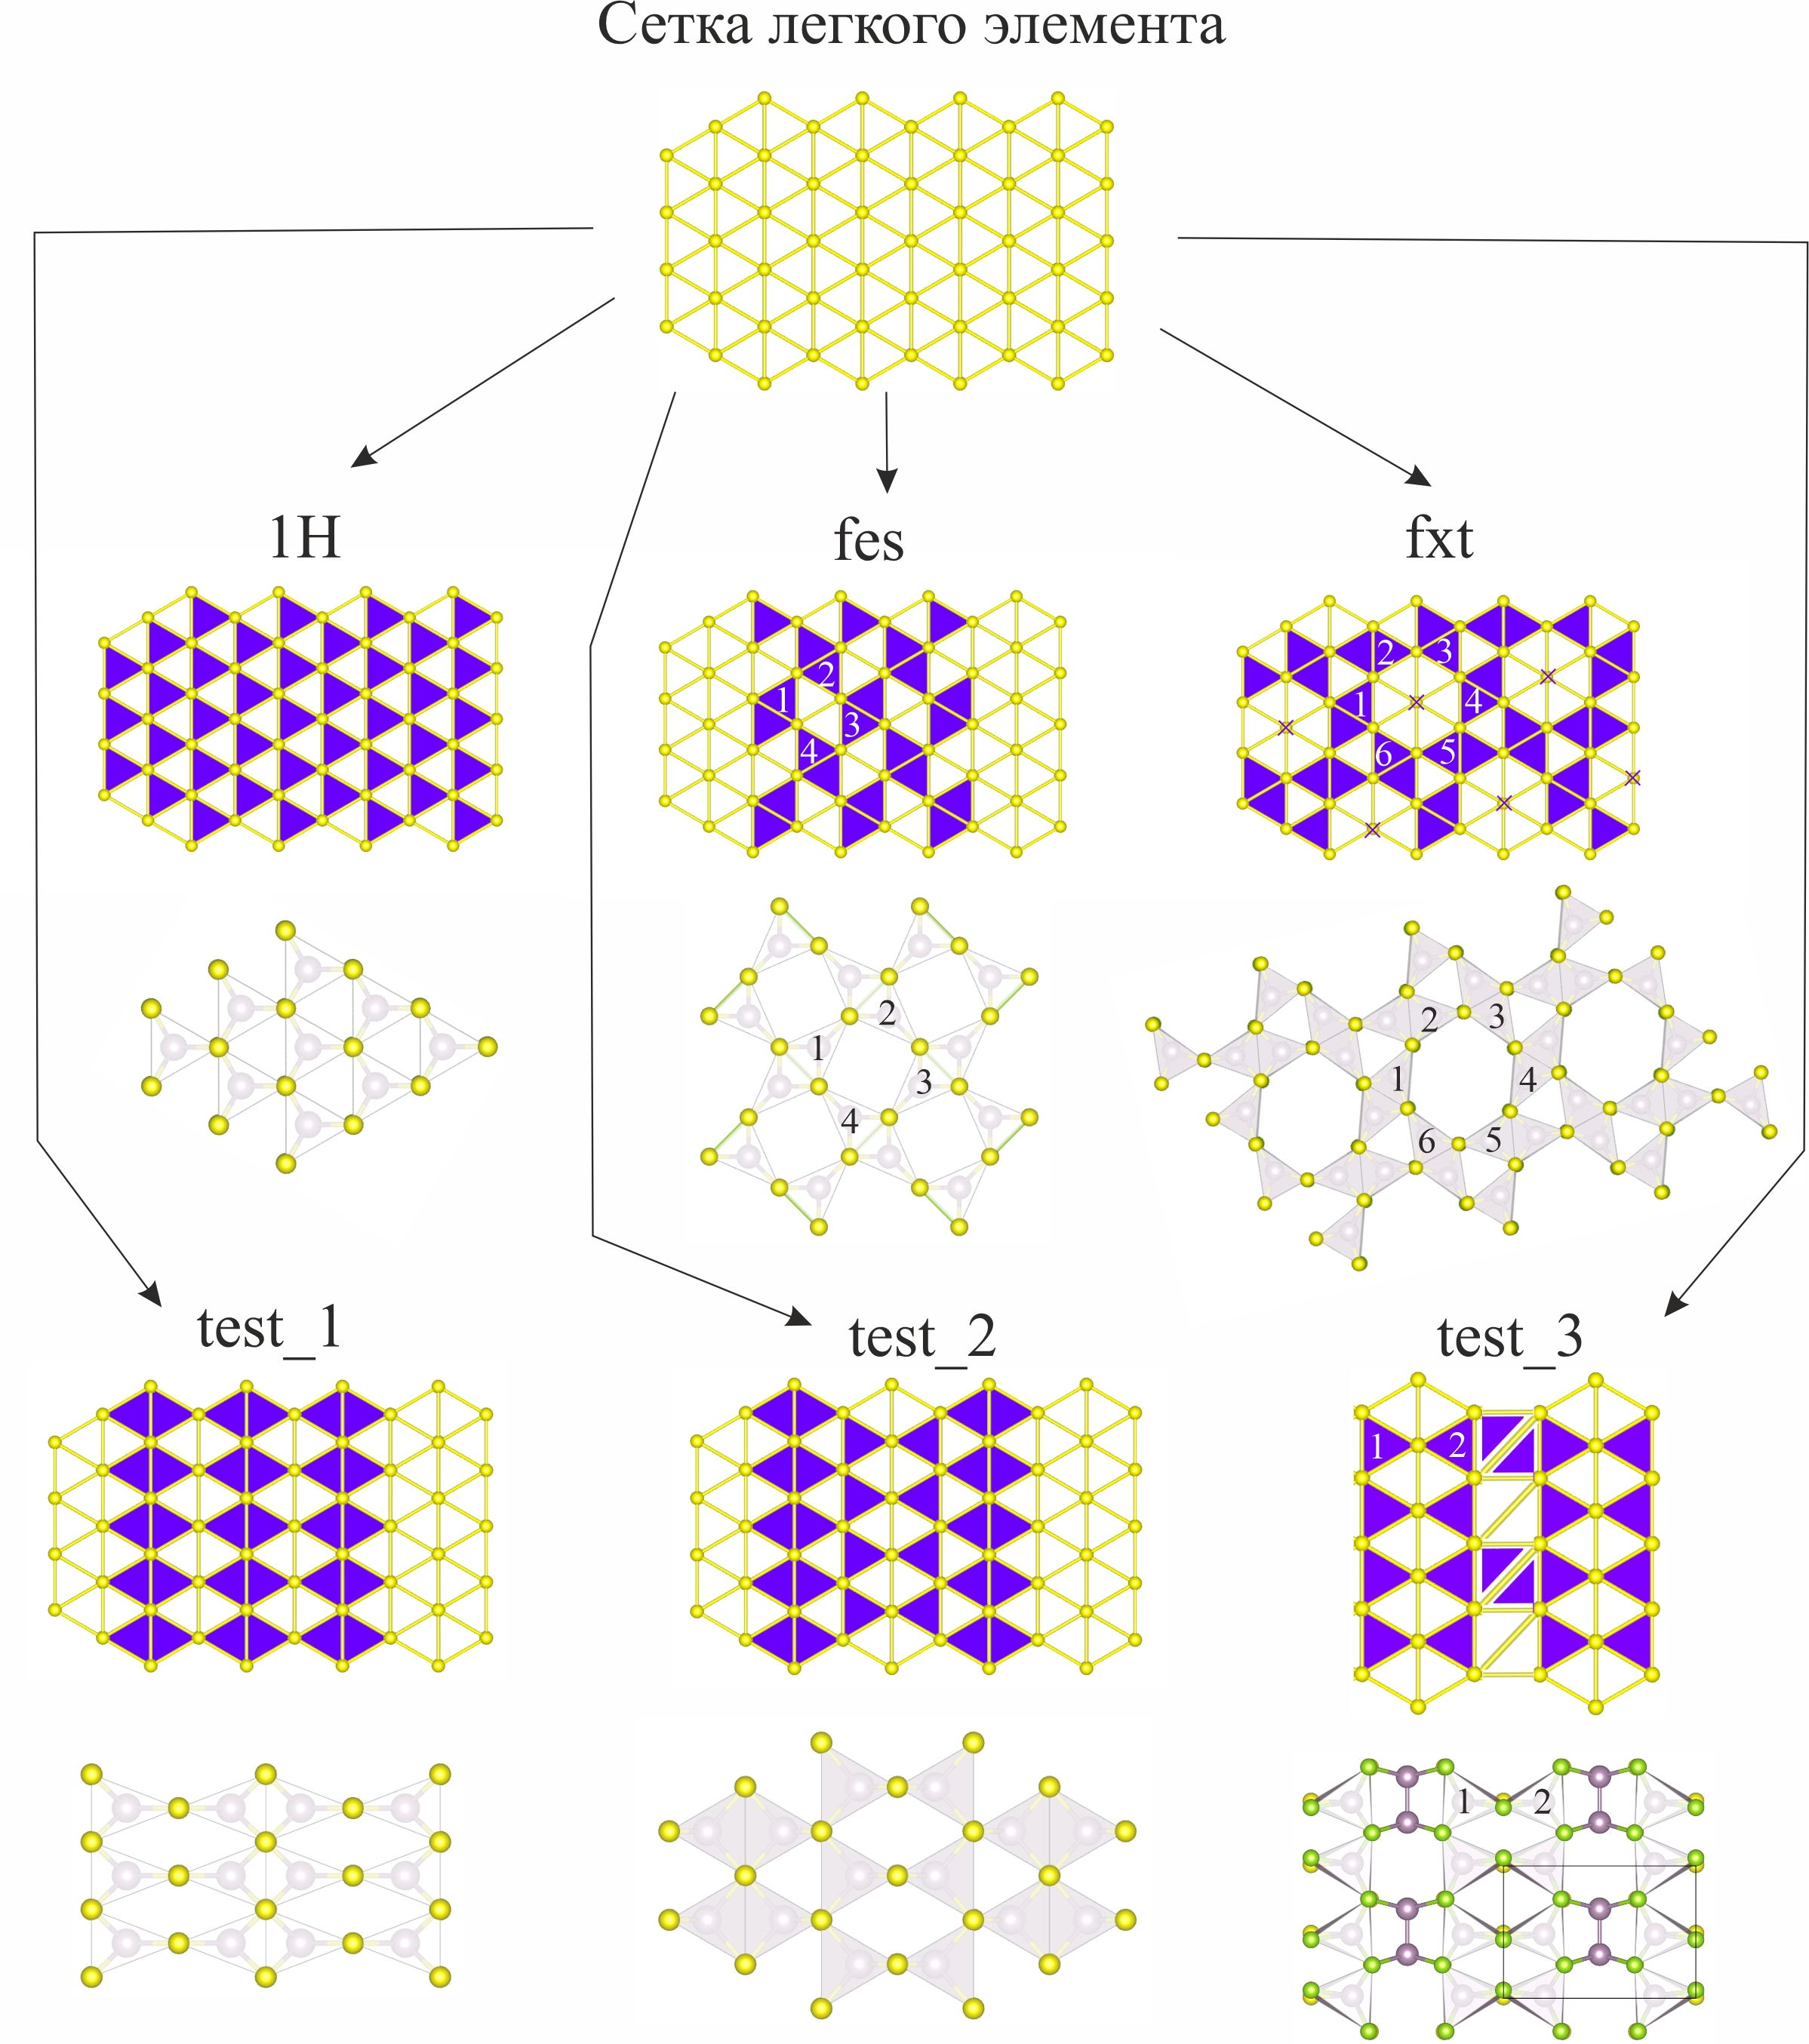
\includegraphics[width=0.8\textwidth]{H-based.jpg}
        \caption{The initial and optimised structures of MoSSe. Тут нужно убрать свзяь Mo-Mo для test3 и вомзможно показать Mo3 в профиль}
\label{H-based}
\end{figure}


Another structure chracterising by trigonal prismatic coordination was found by means of USPEX code.
It is sufficiently different from all the considered above structures in that three-fold axes of trigonal prisms are parallel to the place of sulphur atoms.
As the result the loops of the net sulphur atoms is not more hexagonal, but square. 
This structure was called H-hor (from H-horisontal)

%%%%%%%%%%%%%%%%%%%%%%%%
\subsubsection{Structures with octahedral coordination}
%%%%%%%%%%%%%%%%%%%%%%%

As it was mentioned above T structure, composed of closely packed octahedra does not give such a flexibility as H-structure, as contact of octahedra through the face results in the corrugation of the plane of sulphur atoms. 
One such a structure with face-shared octahedra have been found with AIRSS code.
In this structure each octahedra have four common edges and one common face.
The presence of the common face results in the sufficient corrugation of the layers of sulphur, in contrast to earlier considered structures.
This structure was called T-hor.

\begin{figure}[H]
	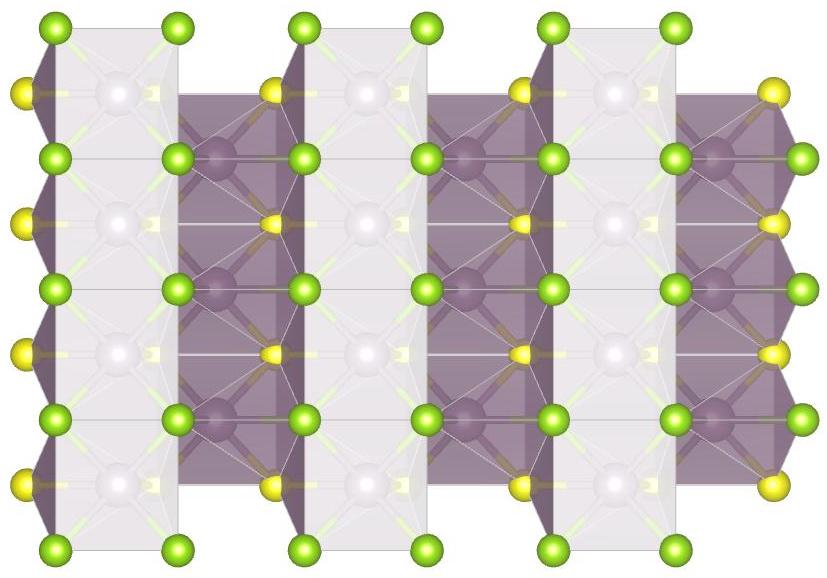
\includegraphics[width=0.75\textwidth]{H_hor_1.jpg} \\
	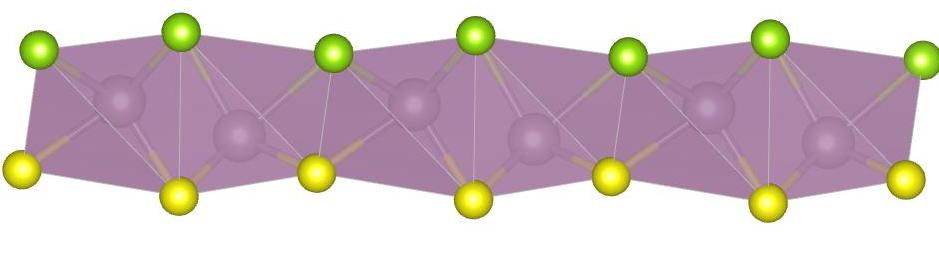
\includegraphics[width=0.75\textwidth]{H_hor_2.jpg}
	\caption{H-hor crystal structure perpendicular and along the layer.}
\label{H_hor}
\end{figure} 


\begin{figure}[H]
        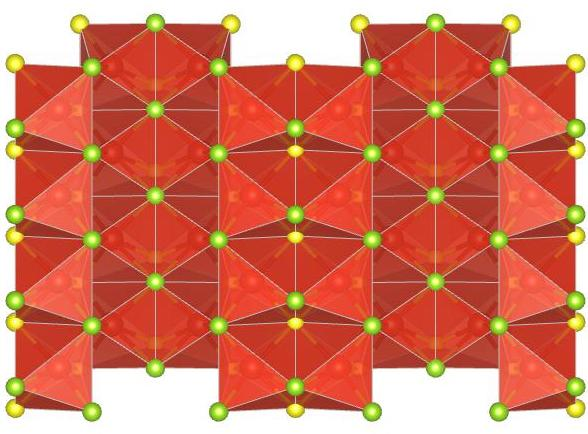
\includegraphics[width=0.75\textwidth]{T_hor_1.jpg} \\
        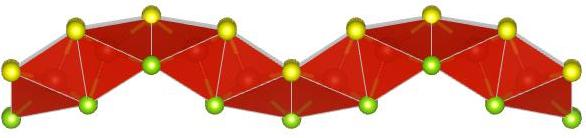
\includegraphics[width=0.75\textwidth]{T_hor_2.jpg}
        \caption{T-hor crystal structure perpendicular and along the layer.}
\label{T_hor}
\end{figure}


%%%%%%%%%%%%%%%%%%%%%%%%
\subsubsection{5-coordinated crystal structure}
%%%%%%%%%%%%%%%%%%%%%%%

Crystal structure with 5-coordinated Mo atoms were revealed with AIRSS code and have been called airss-1.
This structure have not analogues with any structures described above.
Mo atoms are surrounded by 5 chacogenes arranged in tetragonal or ditrigonal pyramids.
Two tetragonal pyramids and one ditrigonal pyramid connected through the edges are grouped in cluters.
The adjacent clusters are connected through the common edges.
Between clusters there are big holes, the sizes of which are comparable with the sizes of the clusters itself.

\begin{figure}[H]
        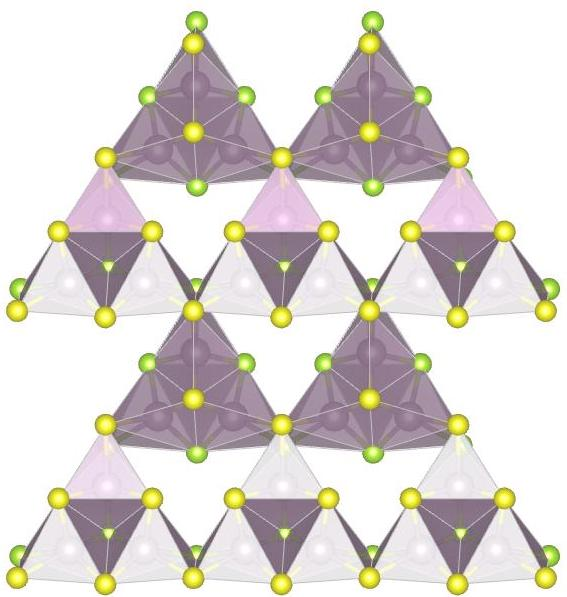
\includegraphics[width=0.75\textwidth]{airss-1-1.jpg} \\ \vspace{3mm}
        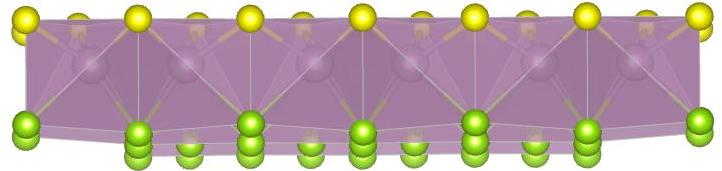
\includegraphics[width=0.75\textwidth]{airss-1-2.jpg}
        \caption{AIRSS-1 structure with 5-coordinated Mo atoms perpendicular and along the layer.}
\label{airss-1}
\end{figure}



%%%%%%%%%%%%%%%%%%%%%%%%
\subsubsection{Crystal structure consisting of mixed layers of TM and Ch (chalcogene)}
%%%%%%%%%%%%%%%%%%%%%%%

The structure in which TM are sufficiently shifted from the center towards upper and bottom layer was revealed for SVSe composition with AIRSS code and have been called airss-3.
V atoms in this structure are characterised by the coordination numbers of five and six, and coordination polyhedron have the forms of tetragonal pyramid and trigonal prism respectively.
Structure can be presented as the combination of double chains, one is with the subhorisontal faces of [SV4] composition in the upper layer and another is with subhorisontal faces of [SeV4] composition in the bottom layer.
Polyhedrons are connected through the common edges.
Each tetragonal pyramid share six out of eight common faces and trigonal pyramid – three out of nein.

\begin{figure}[H]
        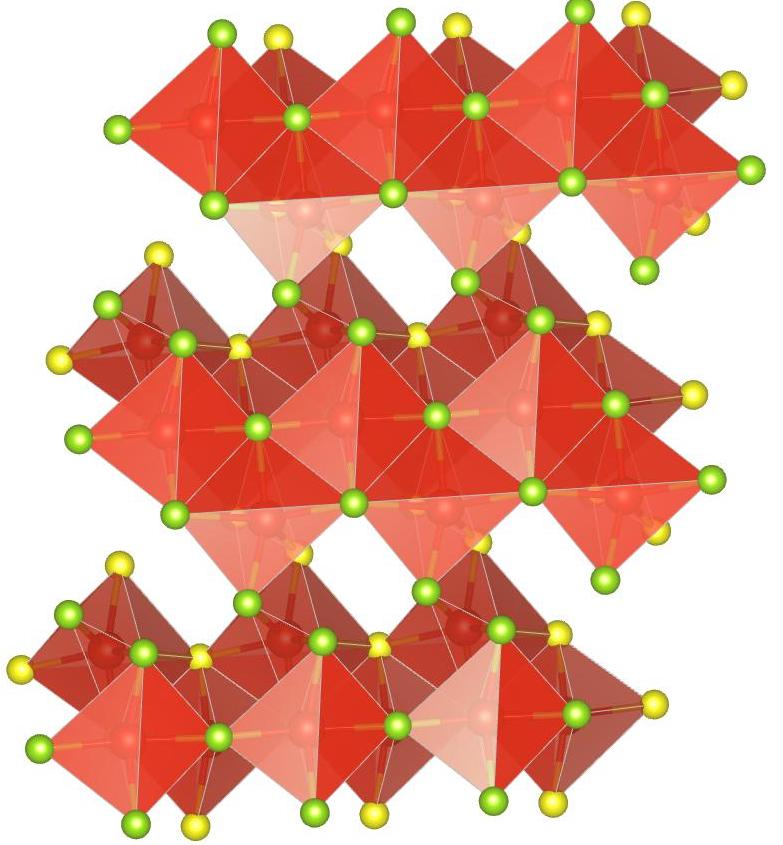
\includegraphics[width=0.75\textwidth]{airss-3-1.jpg} \\ \vspace{3mm}
        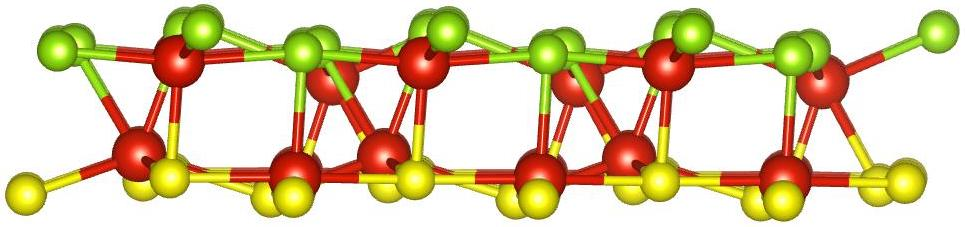
\includegraphics[width=0.75\textwidth]{airss-3-2.jpg}
        \caption{AIRSS-3 structure with V atoms shifted towards the planes of chalcogenes.}
\label{airss-1}
\end{figure}


%%%%%%%%%%%%%%%%%%%%%%%%
\subsubsection{The uniquenes of the new structures}
%%%%%%%%%%%%%%%%%%%%%%%

To answer the question, whether the found structures are unique or there are similar representatives in ICSD we have performed topological search.
The obtained results have shown that all the found structures, except of H-hor, are unique and similar structures are not found in ICSD.
The same is true about the earlier known fxt and fes structures, similar structures of which have not also been found. 
The H-hor structure belong to the same kgd topological type as the T structure.
This mean that one structure can be transformed into another without breaking of the bonds.
However the geometrical difference of H-hor and T structures is sufficient and transformation of one structure into the other requires changing of the coordination polyhedron from trigonal prism to octahedron.

Comment:
Although TOPOS have not found such a structures, some analogues exist.
Interestingly, we note that this structure resembles the structure of the recent experimentally identified monolayer C2N-h2D[J. Mahmood, E. K. Lee, M. Jung, D. Shin, I. Jeon, S. Jung, H. Choi, J. Seo, S. Bae, S. Sohn, N. Park, J. H. Oh, H. Shin, and J.
Baek, Nat. Commun. 6, 6486 (2015)]

\subsection{Stability of the predicted structures}

\begin{table}[h]
	\caption{Calculated enthalpies of SMoSe and SVSe structures.} \label{t:enthalpy} \vspace{2mm}
	\centering
	\begin{tabular}{l*{5}{l}}
		\hline \hline
		\multirow{2}*{Phase} & \multicolumn{2}{c}{Enthalpy (eV/f.u.)} & \multicolumn{2}{c}{Relative H (eV/f.u.)}	\\
		\cline{2-3} \cline{4-5}
		& SMoSe & SVSe & SMoSe & SVSe\\
		\hline    		
		1H	&	-20.8588	&	-15.7908	&	0.0000	&	0.2022	\\
		1T	&	-20.1229	&	-15.8817	&	0.7358	&	0.1113	\\
		1T'	&	-20.4272	&	-15.9930	&	0.4315	&	0.0000	\\
		fes	&	-20.0677	&	-15.3545	&	0.7910	&	0.6385	\\
		fxt	&	-20.0572	&	-15.2915	&	0.8016	&	0.7015	\\
		test-1	&	-19.7876	&	-15.2359	&	1.0711	&	0.7571	\\
		test-2	&	-20.2611	&	-15.4713	&	0.5977	&	0.5217	\\
		test-3	&	-19.9359	&	-15.5461	&	0.9229	&	0.4468	\\
		H-hor	&	-20.0648	&	-15.7256	&	0.7939	&	0.2674	\\
		T-hor	&	-20.3004	&	-15.9091	&	0.5584	&	0.0838	\\
		airss-1	&	-20.2308	&	-15.6641	&	0.6280	&	0.3289	\\
		airss-3	&		        &	-15.6467	&	     	&	0.3463	\\
		
		\hline \hline
	\end{tabular}
\end{table}


\begin{figure}[H]
	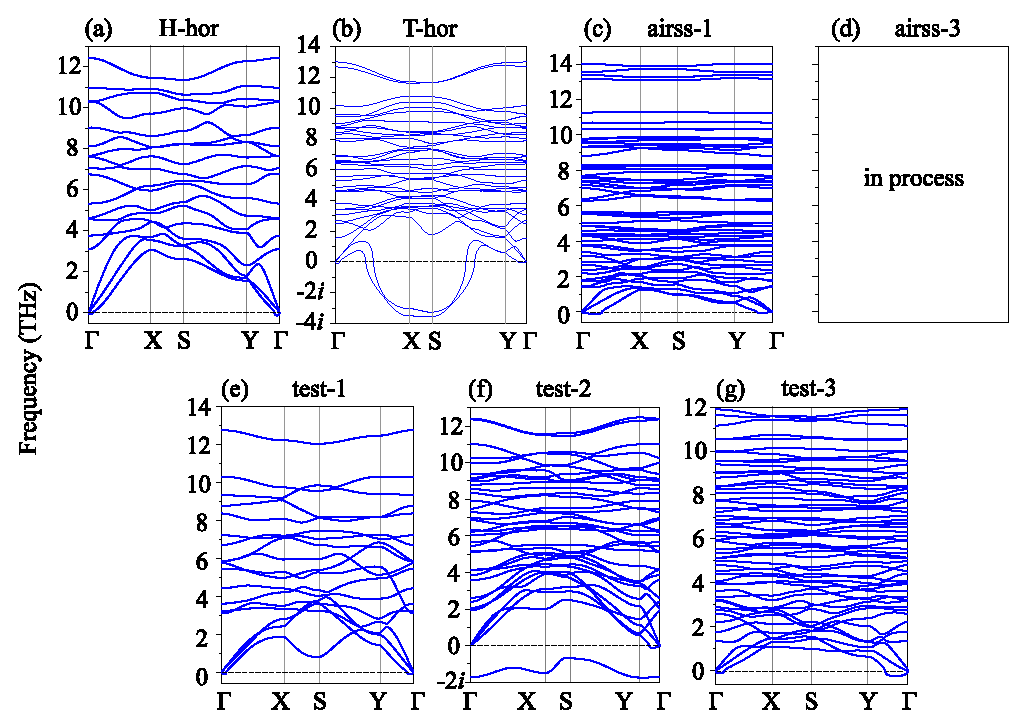
\includegraphics[width=\textwidth]{phon_smose.eps}
	\caption{Phonon dispersion curves of SMoSe structures. }
	\label{phon_smose}
\end{figure}

\begin{figure}[H]
	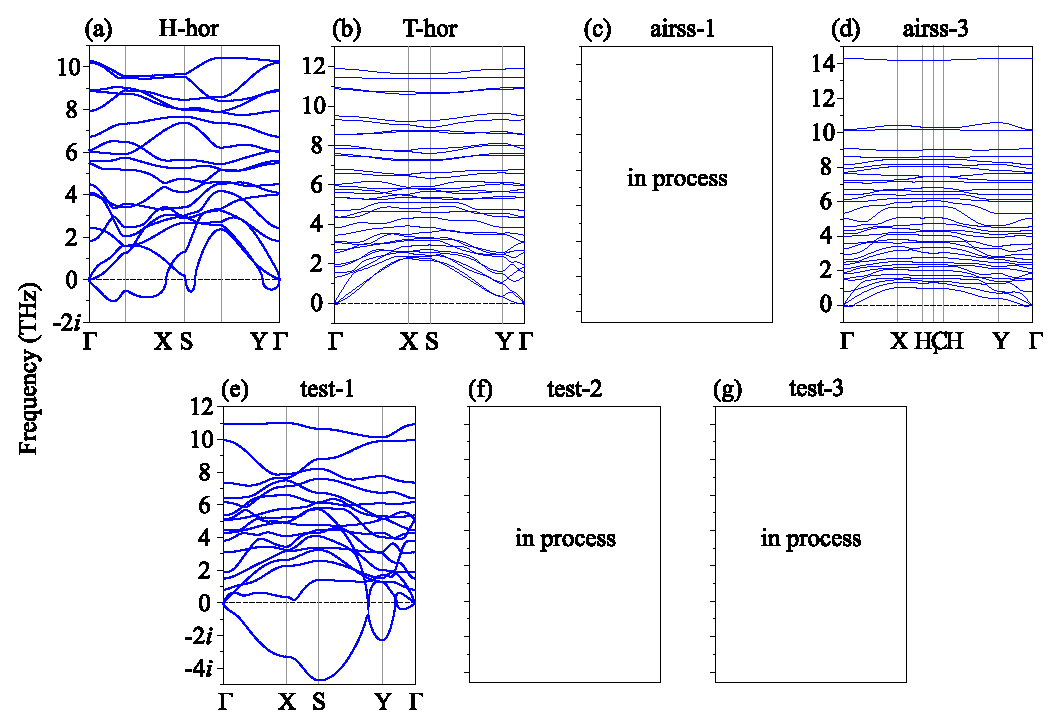
\includegraphics[width=\textwidth]{phon_svse.eps}
	\caption{Phonon dispersion curves of SVSe structures. }
	\label{phon_svse}
\end{figure}


\bibliography{2d}
\bibliographystyle{CGD}


\end{document}


